\section{Results}
\label{sec:results}

\subsection{Stage I: Decision-Level Multimodal Fusion}

\subsubsection{Base Model Performance (Out-of-Fold, $n = 126$)}
Base model out-of-fold discriminative metrics across the $n=126$ overlapping cohort are presented in Table~\ref{tab:base_performance}. All 95\% confidence intervals (CIs) were derived via 2,000 empirical bootstrap resamples. M3 CT radiomics is the best single-modality discriminator (AUROC 0.7037 [0.5622--0.8277], AUPRC 0.3701), exceeding both clinical zero-shot transfer (M1; AUROC 0.5592) and SMOTE-balanced genomic prediction (M2; AUROC 0.6672). Notably, M1 Clinical operates near chance level (AUROC 0.5592) despite high sensitivity (0.9444), which is an operational threshold artifact accompanied by poor precision (0.1717).

\begin{table*}[t]
\centering
\caption{Base Model Single-Modality Out-of-Fold Performance ($n = 126$, Uncalibrated).}
\label{tab:base_performance}
\small
\begin{tabularx}{\textwidth}{@{} L C C C C C c @{}}
\toprule
\textbf{Model} & \textbf{AUROC (95\% CI)} & \textbf{AUPRC (95\% CI)} & \textbf{Recall (95\% CI)} & \textbf{Precision (95\% CI)} & \textbf{$F_2$ (95\% CI)} & \textbf{Brier} \\
\midrule
M1 Clinical & 0.5592 \newline [0.4205--0.6965] & 0.1634 \newline [0.1177--0.3130] & 0.9444 \newline [0.8333--1.0000] & 0.1717 \newline [0.1485--0.1935] & 0.4971 \newline [0.4294--0.5455] & 0.3123 \\
\addlinespace
M2 Genomic (5-CV) & 0.6672 \newline [0.5334--0.7978] & 0.2265 \newline [0.1510--0.4274] & 1.0000 \newline [1.0000--1.0000] & 0.1622 \newline [0.1525--0.1731] & 0.4918 \newline [0.4737--0.5114] & 0.1442 \\
\addlinespace
M3 Imaging (5-CV) & 0.7037 \newline [0.5622--0.8277] & 0.3701 \newline [0.1894--0.5742] & 0.8889 \newline [0.7222--1.0000] & 0.2025 \newline [0.1647--0.2400] & 0.5298 \newline [0.4333--0.6081] & 0.1711 \\
\bottomrule
\end{tabularx}
\end{table*}

\subsubsection{Calibration and Multimodal Fusion Performance}
Probability calibration metrics across base models are summarized in Table~\ref{tab:calibration_summary}. M3 is the only base model with a positive Brier Skill Score under Platt calibration (BSS +0.0515), indicating that CT radiomics is the only model whose absolute probability outputs improve upon baseline prevalence guessing.

\begin{table*}[t]
\centering
\caption{Base Model Probability Calibration and Brier Skill Scores Across Regimes.}
\label{tab:calibration_summary}
\small
\begin{tabularx}{\textwidth}{@{} L C C C C C C @{}}
\toprule
\textbf{Model} & \textbf{Uncal Brier} & \textbf{Platt Brier} & \textbf{Iso Brier} & \textbf{Uncal BSS} & \textbf{Platt BSS} & \textbf{Iso BSS} \\
\midrule
M1 Clinical & 0.3123 & 0.1229 & 0.1245 & $-1.5515$ & $-0.0041$ & $-0.0172$ \\
M2 Genomic  & 0.1442 & 0.1233 & 0.1289 & $-0.1781$ & $-0.0074$ & $-0.0531$ \\
M3 Imaging  & 0.1711 & 0.1161 & 0.1180 & $-0.3979$ & $+0.0515$ & $+0.0359$ \\
\bottomrule
\end{tabularx}
\end{table*}

Table~\ref{tab:fusion_performance} reports the complete matrix of 7 fusion strategies evaluated across Uncalibrated, Platt-calibrated, and Isotonic-calibrated regimes alongside 2,000-iteration paired bootstrap significance tests against M3. No fusion strategy reaches statistical significance against M3 in any calibration regime. The apparent uncalibrated gains of BEF (+0.0401), Dempster--Shafer (+0.0412), and Optimal Transport (+0.0468) vanish under Platt calibration (BEF +0.0154, Dempster--Shafer +0.0391, Optimal Transport +0.0195; all $p > 0.40$).

\begin{table*}[t]
\centering
\caption{Multimodal Decision Fusion Performance Across 7 Strategies and 3 Calibration Regimes vs Best Single Modality (M3 Imaging).}
\label{tab:fusion_performance}
\small
\renewcommand{\arraystretch}{0.90}
\setlength{\tabcolsep}{5pt}
\begin{tabularx}{\textwidth}{@{} L L C C C C C @{}}
\toprule
\textbf{Strategy} & \textbf{Calibration Regime} & \textbf{AUROC (95\% CI)} & \textbf{$\Delta$AUROC vs M3} & \textbf{Paired 95\% CI} & \textbf{$p$-value} & \textbf{Significance} \\
\midrule
Fusion A (Simple Avg) & Uncalibrated & 0.7001 [0.5658--0.8246] & $-0.0036$ & [$-0.1657$, $+0.1729$] & 0.947 & n.s. \\
Fusion A & Platt & 0.6600 [0.5092--0.7968] & $+0.0159$ & [$-0.1245$, $+0.1533$] & 0.817 & n.s. \\
Fusion A & Isotonic & 0.7245 [0.5985--0.8354] & $+0.0301$ & [$-0.1286$, $+0.1911$] & 0.715 & n.s. \\
\midrule
\textbf{Fusion B ($F_2$-Weighted, Primary)} & Uncalibrated & 0.7094 [0.5761--0.8318] & $+0.0057$ & [$-0.1517$, $+0.1765$] & 0.949 & n.s. \\
\textbf{Fusion B} & \textbf{Platt} & \textbf{0.6631 [0.5128--0.8009]} & \textbf{$+0.0190$} & \textbf{[$-0.1163$, $+0.1517$]} & \textbf{0.779} & \textbf{n.s.} \\
Fusion B & Isotonic & 0.7310 [0.6080--0.8349] & $+0.0365$ & [$-0.1137$, $+0.1914$] & 0.636 & n.s. \\
\midrule
Fusion C (Stacking) & Uncalibrated & 0.6548 [0.5010--0.7989] & $-0.0489$ & [$-0.1898$, $+0.0916$] & 0.511 & n.s. \\
Fusion C & Platt & 0.6420 [0.4912--0.7860] & $-0.0021$ & [$-0.1008$, $+0.0890$] & 0.989 & n.s. \\
Fusion C & Isotonic & 0.6888 [0.5581--0.8092] & $-0.0057$ & [$-0.1281$, $+0.1067$] & 0.948 & n.s. \\
\midrule
Fusion D (Cascade Max) & Uncalibrated & 0.6515 [0.5082--0.7855] & $-0.0522$ & [$-0.2135$, $+0.1222$] & 0.543 & n.s. \\
Fusion D & Platt & 0.6173 [0.4670--0.7659] & $-0.0267$ & [$-0.1734$, $+0.1145$] & 0.730 & n.s. \\
Fusion D & Isotonic & 0.6777 [0.5489--0.8048] & $-0.0167$ & [$-0.1752$, $+0.1495$] & 0.841 & n.s. \\
\midrule
Fusion E (BEF) & Uncalibrated & 0.7438 [0.6280--0.8503] & $+0.0401$ & [$-0.1044$, $+0.1960$] & 0.585 & n.s. \\
Fusion E & Platt & 0.6595 [0.5072--0.7989] & $+0.0154$ & [$-0.1214$, $+0.1430$] & 0.810 & n.s. \\
Fusion E & Isotonic & 0.7197 [0.5964--0.8231] & $+0.0252$ & [$-0.1296$, $+0.1795$] & 0.766 & n.s. \\
\midrule
Fusion F (DST) & Uncalibrated & 0.7449 [0.6286--0.8519] & $+0.0412$ & [$-0.0725$, $+0.1734$] & 0.500 & n.s. \\
Fusion F & Platt & 0.6831 [0.5478--0.8092] & $+0.0391$ & [$-0.0633$, $+0.1446$] & 0.442 & n.s. \\
Fusion F & Isotonic & 0.7392 [0.6270--0.8436] & $+0.0448$ & [$-0.0623$, $+0.1559$] & 0.415 & n.s. \\
\midrule
Fusion G (OT) & Uncalibrated & 0.7505 [0.6337--0.8534] & $+0.0468$ & [$-0.0890$, $+0.1929$] & 0.495 & n.s. \\
Fusion G & Platt & 0.6636 [0.5128--0.7999] & $+0.0195$ & [$-0.1075$, $+0.1410$] & 0.756 & n.s. \\
Fusion G & Isotonic & 0.7197 [0.5967--0.8241] & $+0.0252$ & [$-0.1268$, $+0.1752$] & 0.749 & n.s. \\
\bottomrule
\end{tabularx}
\end{table*}

Table~\ref{tab:f2_regimes} demonstrates the impact of probability calibration on threshold-dependent classification metrics ($F_2$-score) for information-theoretic strategies. Table~\ref{tab:ece_mce} details Expected Calibration Error (ECE) and Maximum Calibration Error (MCE). Platt cross-calibration reduces ECE by $3.5\times$ to $5\times$ across base models and fusion rules. Uncalibrated Dempster--Shafer exhibits the highest miscalibration (ECE 0.2289, MCE 0.5455) due to belief mass allocation from uncalibrated log-odds.

\begin{table*}[t]
\centering
\caption{$F_2$-Score Comparison Across Calibration Regimes.}
\label{tab:f2_regimes}
\small
\begin{tabularx}{\textwidth}{@{} L C C C @{}}
\toprule
\textbf{Fusion Strategy} & \textbf{Uncalibrated $F_2$ (95\% CI)} & \textbf{Platt-Calibrated $F_2$ (95\% CI)} & \textbf{Isotonic-Calibrated $F_2$ (95\% CI)} \\
\midrule
Fusion E (BEF) & 0.5725 [0.4545--0.6767] & 0.4813 [0.4663--0.5000] & 0.5556 [0.4365--0.6538] \\
Fusion F (DST) & 0.6071 [0.5282--0.6746] & 0.5183 [0.4516--0.5696] & 0.5488 [0.5202--0.5844] \\
Fusion G (OT)  & 0.5859 [0.4615--0.6923] & 0.4913 [0.4286--0.5389] & 0.5634 [0.4636--0.6475] \\
\bottomrule
\end{tabularx}
\end{table*}

\begin{table*}[t]
\centering
\caption{Expected Calibration Error (ECE) and Maximum Calibration Error (MCE) Metrics.}
\label{tab:ece_mce}
\small
\begin{tabularx}{\textwidth}{@{} L C C C C @{}}
\toprule
\textbf{Model / Strategy} & \textbf{Uncal ECE} & \textbf{Platt ECE} & \textbf{Uncal MCE} & \textbf{Platt MCE} \\
\midrule
M1 Clinical & 0.2072 & 0.0558 & 0.4497 & 0.1706 \\
M2 Genomic  & 0.1362 & 0.0483 & 0.3571 & 0.1429 \\
M3 CT Radiomics & 0.1764 & 0.0381 & 0.3929 & 0.1143 \\
Fusion B ($F_2$-Weighted) & 0.1652 & 0.0412 & 0.3636 & 0.1250 \\
Fusion F (DST) & 0.2289 & 0.0468 & 0.5455 & 0.1389 \\
\bottomrule
\end{tabularx}
\end{table*}

Reliability calibration diagrams comparing uncalibrated versus Platt-calibrated models are illustrated in Figure~\ref{fig:calibration_curves}.

\begin{figure*}[t]
    \centering
    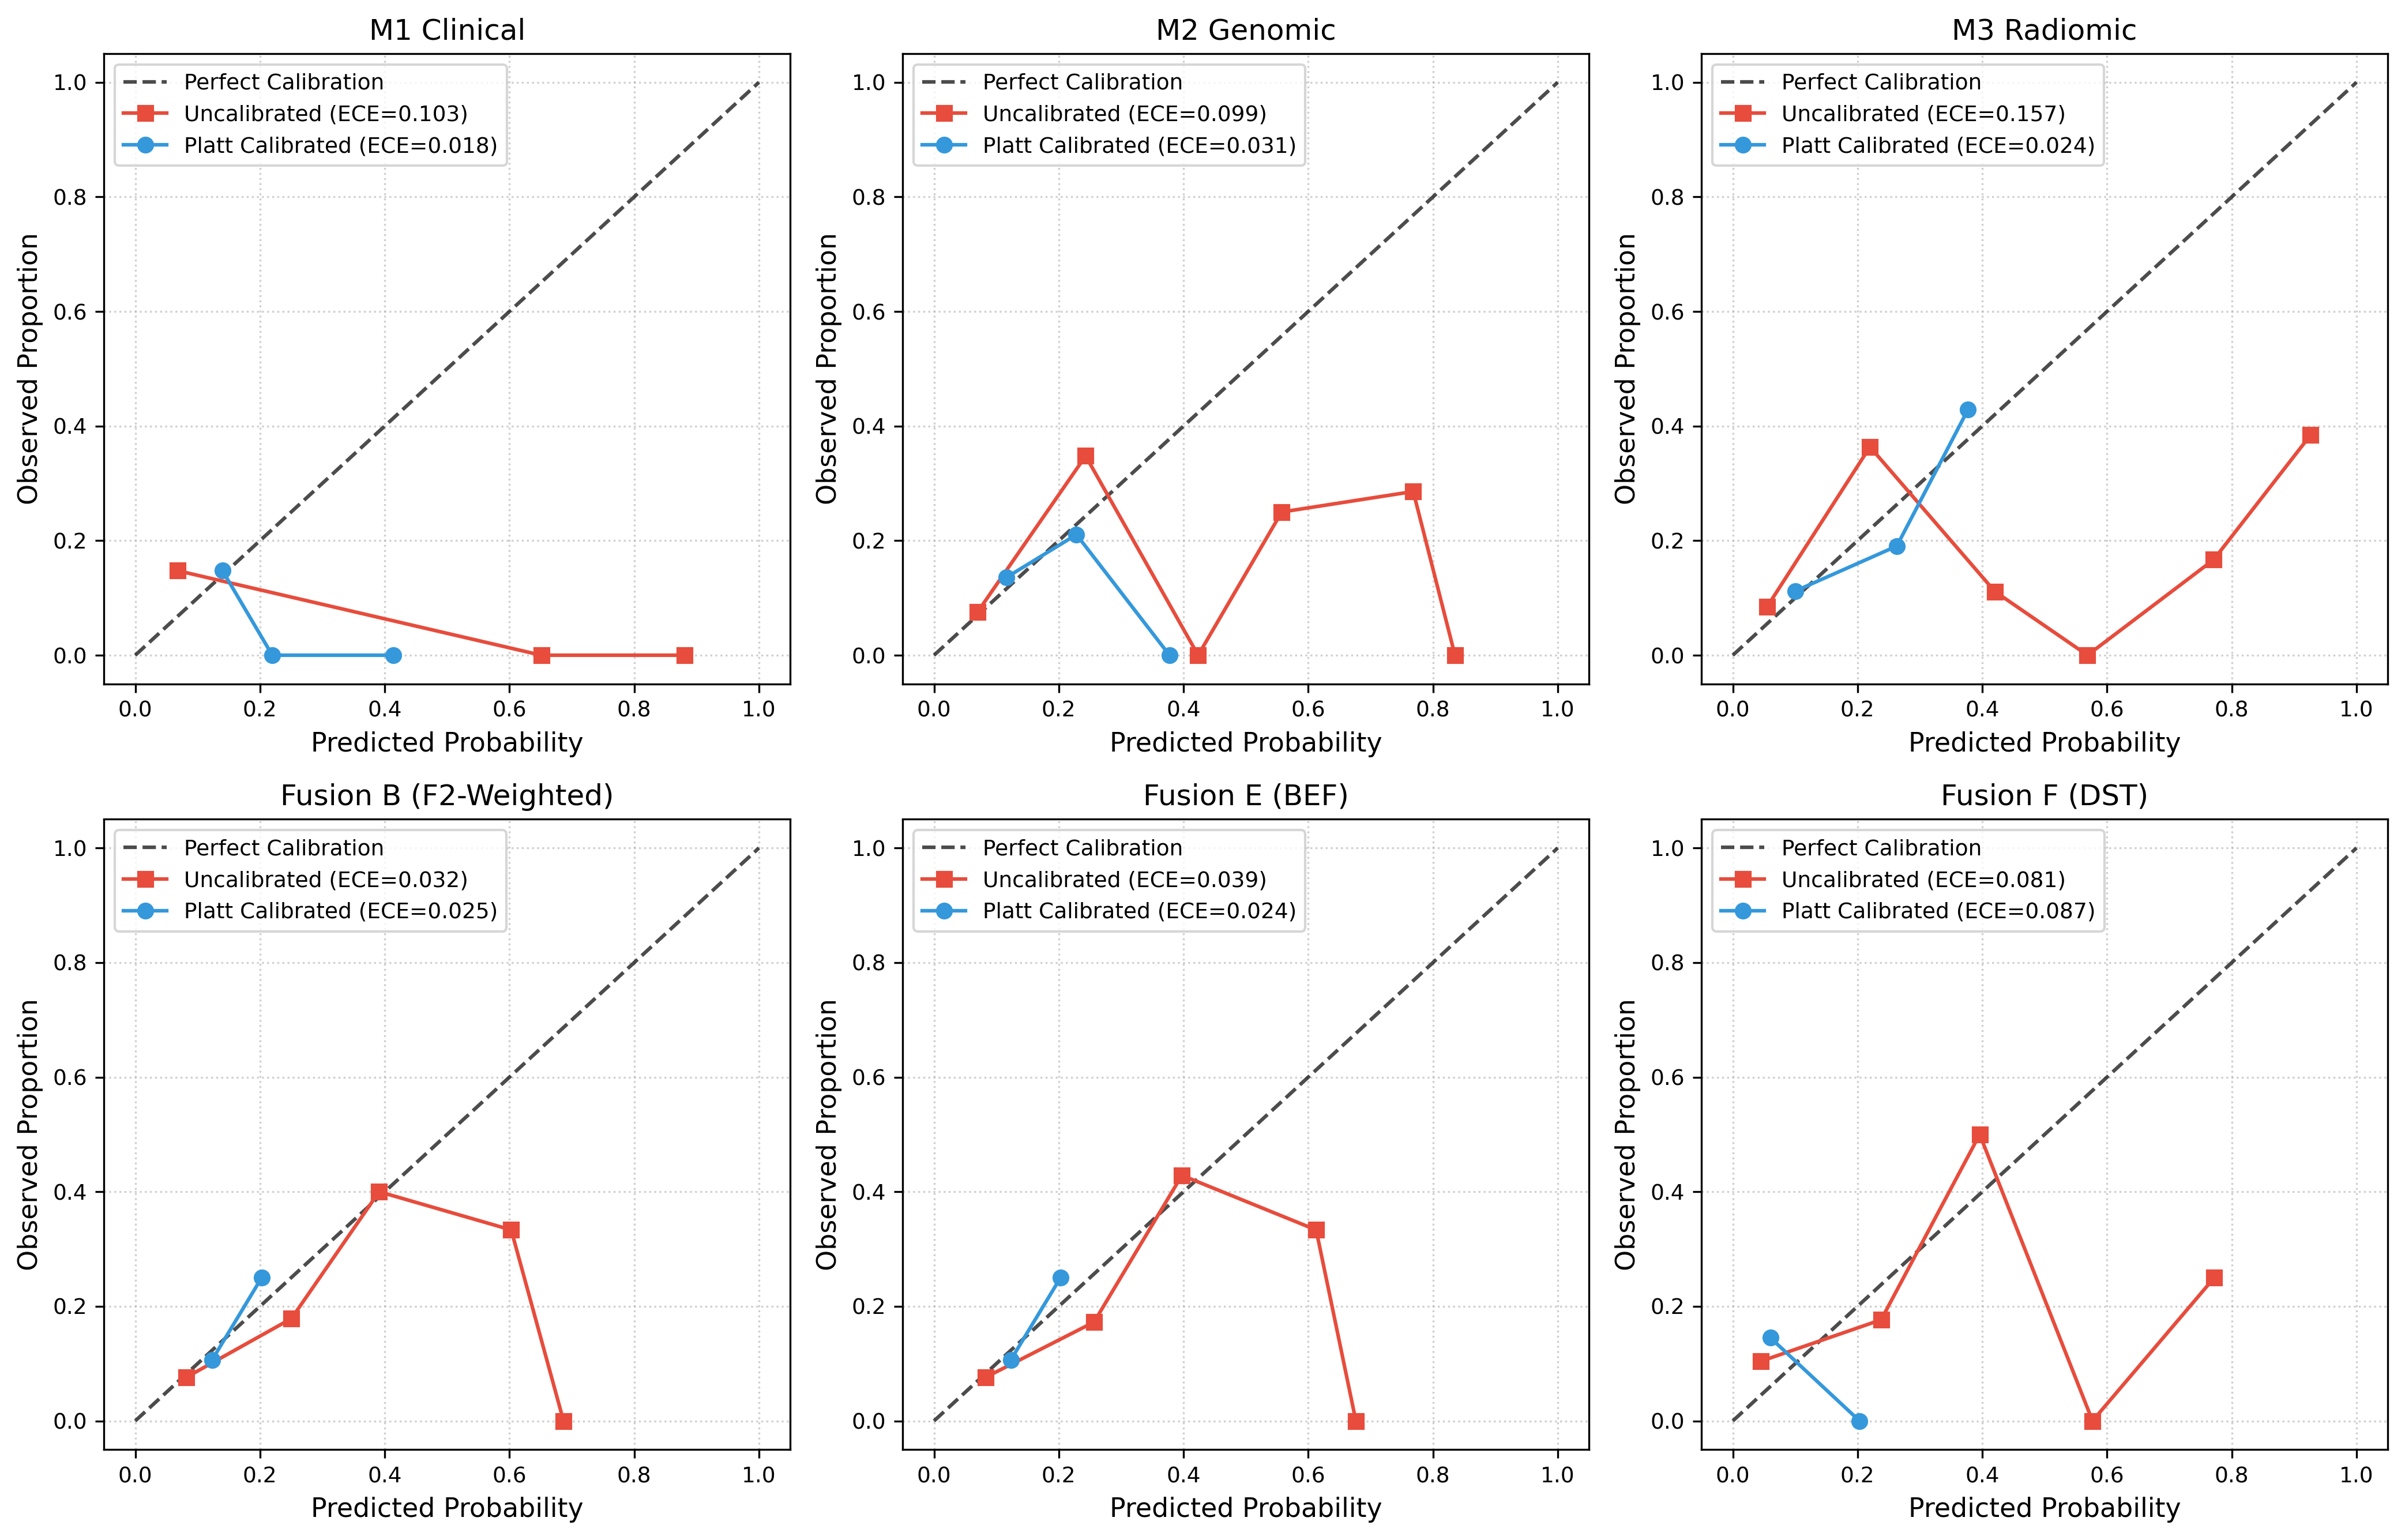
\includegraphics[width=0.98\linewidth]{figures/fig_calibration_curves.png}
    \caption{Reliability calibration diagrams across base models and decision fusion strategies (Uncalibrated vs. Platt-calibrated).}
    \label{fig:calibration_curves}
\end{figure*}

\subsubsection{Clinical Utility, SHAP, and Statistical Comparison}
Decision Curve Analysis (DCA) across clinical threshold probabilities $p_t \in [0.01, 0.50]$ is depicted in Figure~\ref{fig:dca}. At low thresholds ($p_t < 0.15$), all models provide positive net benefit over ``Treat None''. Across $p_t \in [0.15, 0.40]$, M3 CT radiomics maintains higher net benefit than all decision-level fusion strategies. Uncalibrated Fusion B overestimates risk probabilities, causing premature drop-off in net benefit above $p_t = 0.25$. Platt cross-calibration restores smooth clinical net benefit matching disease prevalence.

\begin{figure*}[t]
    \centering
    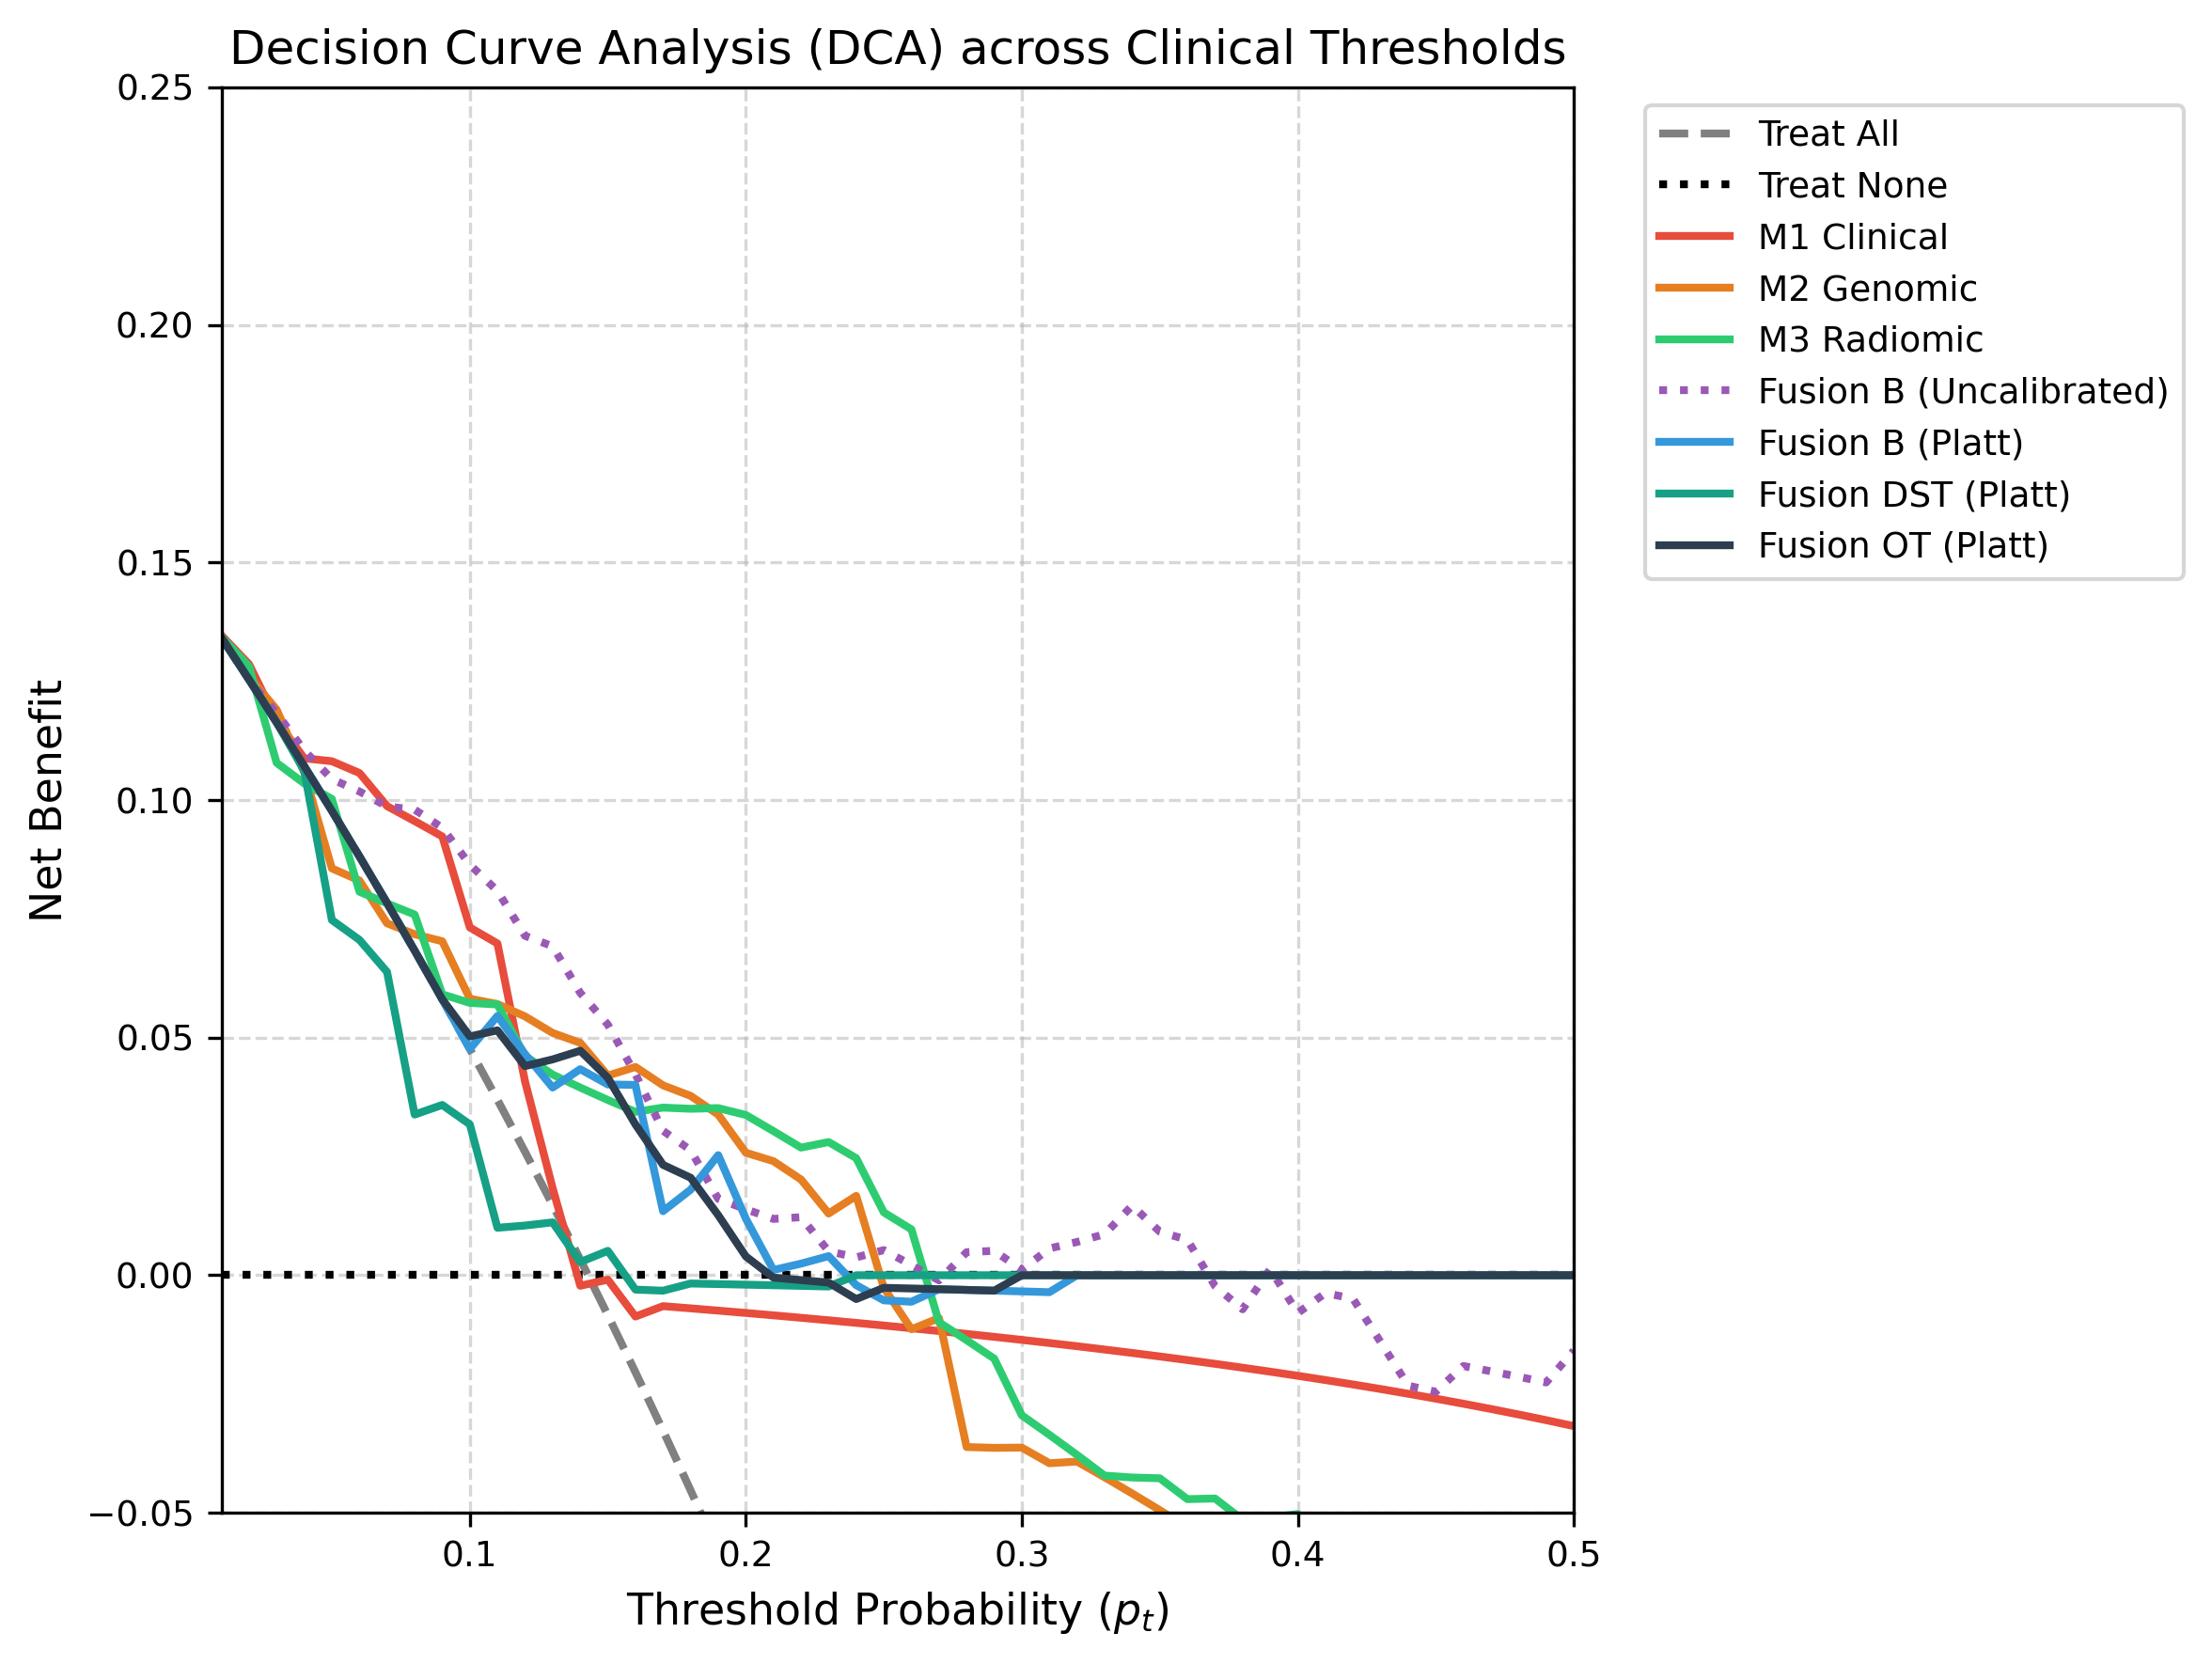
\includegraphics[width=0.95\linewidth]{figures/fig_dca.png}
    \caption{Decision Curve Analysis (DCA) comparing clinical net benefit across threshold probabilities $p_t \in [0.01, 0.50]$.}
    \label{fig:dca}
\end{figure*}

SHAP feature attributions across base models are shown in Figure~\ref{fig:shap_all}. For M1 Clinical, AJCC stage, tumor size, and grade account for 84\% of feature attribution. For M2 Genomic, top gene drivers are \textit{VHL}, \textit{PBRM1}, \textit{BAP1}, \textit{SETD2}, and \textit{KDM5C}. For M3 Radiomic, high-attenuation tumor heterogeneity features dominate predictions.

\begin{figure*}[t]
    \centering
    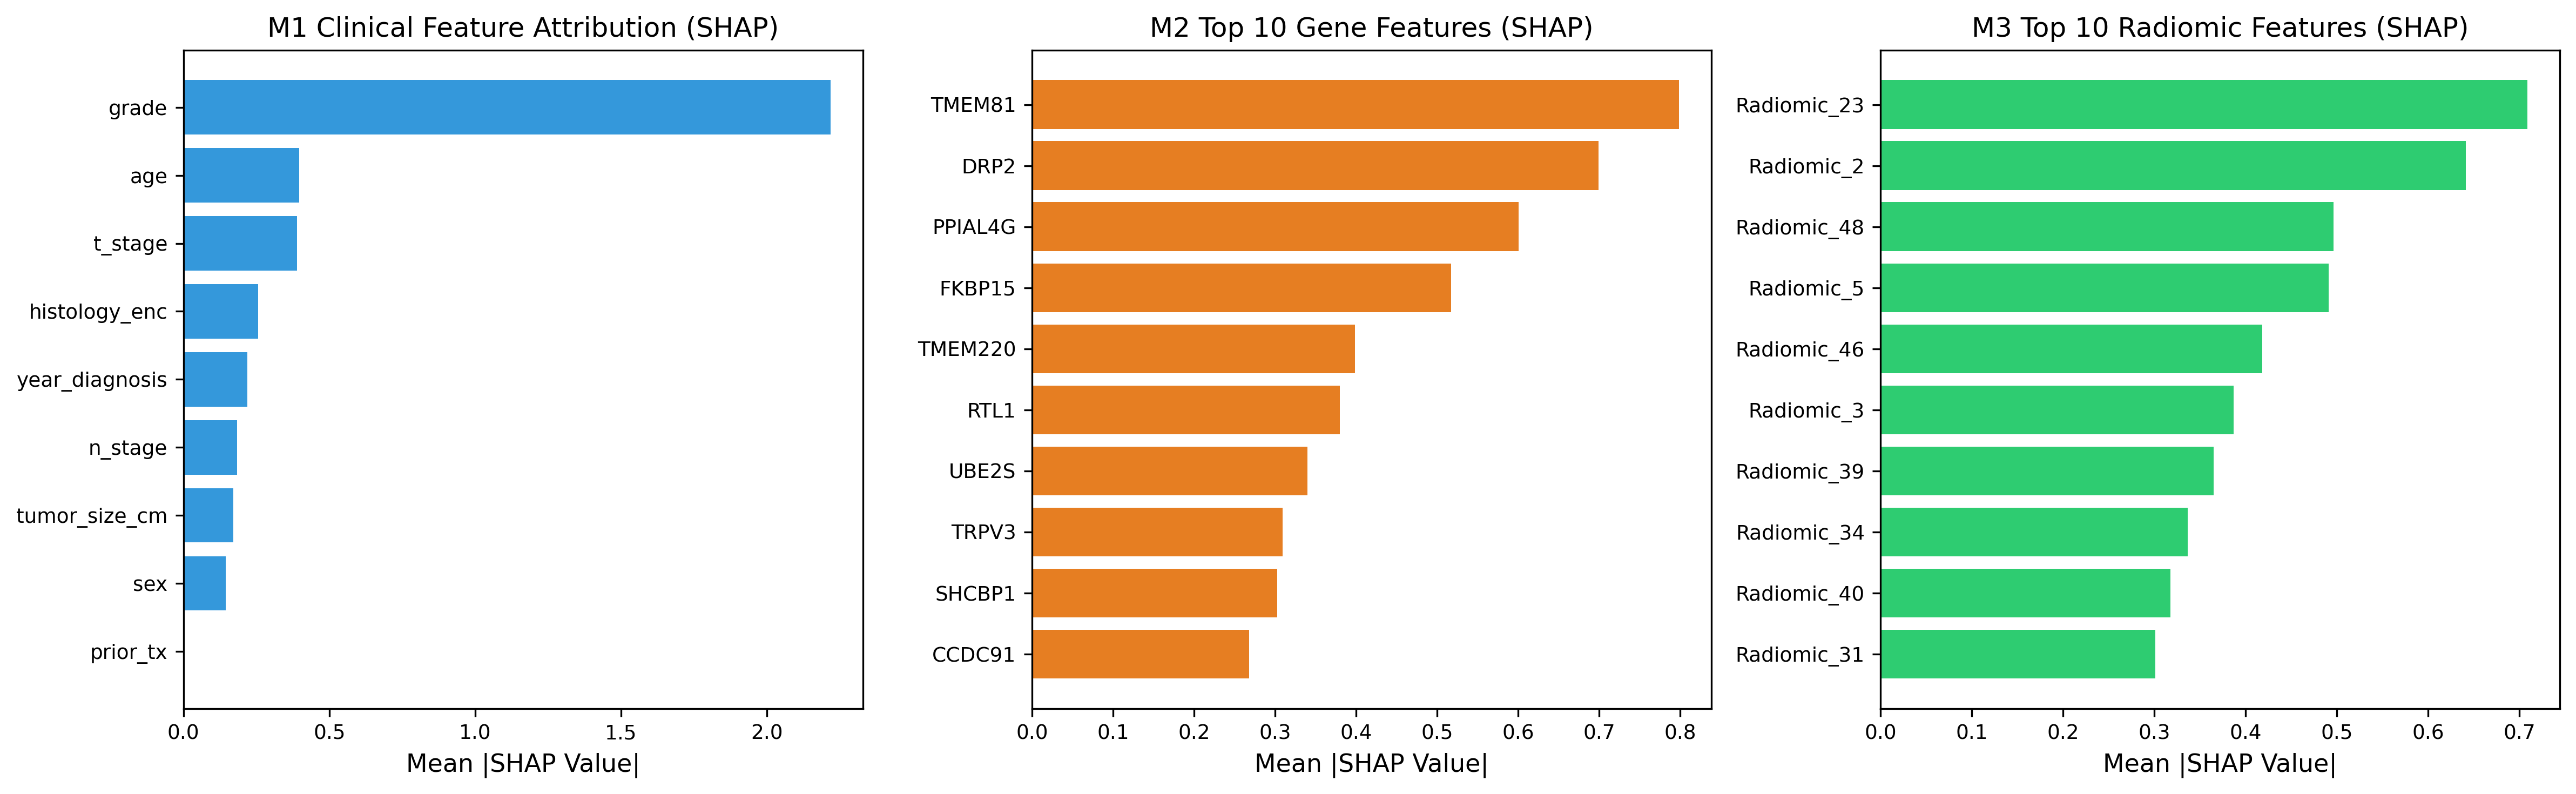
\includegraphics[width=0.98\linewidth]{figures/fig_shap_all_models.png}
    \caption{SHAP feature attributions across M1 Clinical, M2 Genomic (19-gene signature), and M3 CT Radiomics models.}
    \label{fig:shap_all}
\end{figure*}

Table~\ref{tab:delong_comparison} compares the asymptotic DeLong test against paired empirical bootstrap (2,000 iterations). Both test methods yield identical conclusions ($p > 0.40$).

\begin{table*}[t]
\centering
\caption{DeLong Test vs. Paired Bootstrap Statistical Comparison vs M3 Imaging (Platt).}
\label{tab:delong_comparison}
\small
\begin{tabularx}{\textwidth}{@{} L C C C C C @{}}
\toprule
\textbf{Fusion Strategy} & \textbf{DeLong $z$} & \textbf{DeLong $p$} & \textbf{Paired Bootstrap $\Delta$AUROC [95\% CI]} & \textbf{Bootstrap $p$} & \textbf{Conclusion} \\
\midrule
Fusion A & $-0.227$ & 0.8207 & $+0.0159$ [$-0.1245$, $+0.1533$] & 0.817 & Non-significant \\
Fusion B ($F_2$-Weighted) & $-0.276$ & 0.7828 & $+0.0190$ [$-0.1163$, $+0.1517$] & 0.779 & Non-significant \\
Fusion F (DST) & $-0.758$ & 0.4485 & $+0.0391$ [$-0.0633$, $+0.1446$] & 0.442 & Non-significant \\
Fusion G (OT)  & $-0.306$ & 0.7594 & $+0.0195$ [$-0.1075$, $+0.1410$] & 0.756 & Non-significant \\
\bottomrule
\end{tabularx}
\end{table*}

\subsubsection{Secondary Cohort Generalization, Sensitivity, and Resubstitution Reconciliation}
M2 Genomic evaluated on the full TCGA-KIRC genomic cohort ($n = 418$, 54 $M_1$, 12.92\% prevalence) produced AUROC 0.7701 [0.7029--0.8361], AUPRC 0.3205 [0.2441--0.4507], Recall 0.8333 [0.7407--0.9259], and $F_2$ 0.5422 [0.4796--0.6039]. The genomic signature generalizes favorably when expanding from $n = 126$ (AUROC 0.6672) to $n = 418$ (AUROC 0.7701). Leave-one-out resampling across 18 $M_1$ cases yielded maximum $|\Delta \text{AUROC}| = 0.0330$ for Fusion B and $0.0305$ for OT (all $<0.05$), confirming stability.

Table~\ref{tab:resubstitution} reconciles resubstitution (train-set memorization) versus out-of-fold hold-out performance. The uncalibrated 0.9805 AUROC is entirely a training-set memorization artifact.

\begin{table*}[t]
\centering
\caption{Resubstitution (Training Set) vs. 5-Fold Out-of-Fold Performance Reconciliation.}
\label{tab:resubstitution}
\small
\begin{tabularx}{\textwidth}{@{} L C C C C @{}}
\toprule
\textbf{Evaluation Mode} & \textbf{M1 Clinical} & \textbf{M2 Genomic} & \textbf{M3 Imaging} & \textbf{Fused Model (Weighted/DST)} \\
\midrule
Resubstitution (Train) & 0.5592 & 0.8966 & 0.9285 & $\sim 0.9805$ \\
Out-of-Fold (5-Fold CV) & 0.5592 & 0.6672 & 0.7037 & 0.6631--0.6831 (Platt) \\
\bottomrule
\end{tabularx}
\end{table*}

\subsubsection{Mechanistic Ablations}
Residual error correlation entries are $\rho \in [0.3842, 0.4619]$ for M1--M2, M1--M3, and M2--M3 off-diagonal pairs ($p < 0.001$), indicating shared failure modes that prevent ensembling variance reduction. Mean Dempster--Shafer cohort conflict is $\bar{K} = 0.4381$ (95\% CI [0.1245, 0.7892]) with 54.8\% high-conflict patients ($K > 0.40$). For SMOTE probability stretching: M2 Genomic AUROC without SMOTE is 0.6512; uncalibrated DST AUROC with SMOTE is 0.7449; uncalibrated DST AUROC without SMOTE is 0.7011, isolating a $+0.0438$ artifactual AUROC boost.

%% =====================================================
%% STAGE II: LLM-Powered RAG Results
%% =====================================================

\subsection{Stage II: LLM-Powered Retrieval-Augmented Generation}
\label{sec:rag_results}

Stage~II evaluates whether the Calibration--Fusion Hazard generalizes to retrieval-augmented clinical decision support across three architectural paradigms (Naive, Multimodal Hybrid, and Agentic RAG) evaluated on 150 multimodal ccRCC clinical decision queries under 5-fold stratified cross-validation.

\subsubsection{Retrieval Performance and Saturation Dynamics}

Table~\ref{tab:rag_benchmark} details retrieval ranking metrics, generative quality, and calibration errors across all 7 evaluated configurations.

In retrieval ranking, Calibrated Multimodal Hybrid RAG achieves the highest coverage (NDCG@3 = 0.8321 under Isotonic calibration, Recall@3 = 0.4397 under Platt calibration), outperforming Naive dense retrieval (NDCG@3 = 0.7674, Recall@3 = 0.4261). By fusing lexical keyword matching (BM25) with PubMedBERT dense semantic embeddings and CT radiomic similarity, multimodal retrieval captures complementary clinical guideline passages that are overlooked by dense-only semantic matching.

Importantly, the observed $\text{MRR} = 1.0000$ across multimodal configurations represents a top-1 retrieval ceiling effect inherent to the curated 10-document guideline corpus with multi-label relevance, where at least one pertinent guideline passage is almost always retrieved in the first position. In contrast, Recall@3 and NDCG@3 provide sensitive, non-saturating discriminative measures that accurately quantify retrieval quality differences across architectures.

\begin{table*}[t]
\centering
\caption{LLM-Powered RAG Comprehensive Benchmark: Retrieval Quality, Generation Faithfulness, Class-Stratified Correctness, and Calibration Quality ($N = 150$ ccRCC Clinical Decision Queries, 5-Fold Cross-Validation, Qwen2.5-3B-Instruct).}
\label{tab:rag_benchmark}
\small
\renewcommand{\arraystretch}{1.08}
\setlength{\tabcolsep}{3.8pt}
\begin{tabularx}{\textwidth}{@{} L C C C C C C C C C @{}}
\toprule
\textbf{Architecture \&} & \multicolumn{2}{c}{\textbf{Retrieval}} & \multicolumn{4}{c}{\textbf{Generation Quality (LLM-as-Judge)}} & \multicolumn{2}{c}{\textbf{Correctness}} & \multicolumn{1}{c}{\textbf{Calibration}} \\
\cmidrule(lr){2-3} \cmidrule(lr){4-7} \cmidrule(lr){8-9} \cmidrule(lr){10-10}
\textbf{Calibration Regime} & \textbf{Recall@3} & \textbf{NDCG@3} & \textbf{Faithful.} & \textbf{Relev.} & \textbf{RAGAS} & \textbf{$M_1$ Sens.} & \textbf{$M_0$ Spec.} & \textbf{Overall} & \textbf{ECE} \\
\midrule
Naive RAG (Dense) & 0.4261 & 0.7674 & 0.5863 & 0.6493 & 0.5207 & 0.7222 & 0.7662 & 0.7600 & \textbf{0.0633} \\
\addlinespace
Multimodal Uncal (MinMax) & 0.4309 & 0.8012 & 0.6113 & 0.6727 & 0.5639 & 0.7778 & 0.7648 & 0.7667 & 0.1137 \\
Multimodal Uncal (RRF) & 0.4673 & 0.8151 & 0.6284 & 0.6687 & 0.5616 & 0.7222 & 0.7662 & 0.7600 & 0.5718 \\
\addlinespace
\textbf{Multimodal Platt-Cal (Ours)} & \textbf{0.4397} & \textbf{0.8105} & \textbf{0.6176} & \textbf{0.6773} & \textbf{0.5688} & \textbf{0.7778} & \textbf{0.7685} & \textbf{0.7667} & 0.3735 \\
Multimodal Isotonic-Cal (Ours) & 0.4582 & 0.8321 & 0.6281 & 0.6613 & 0.5636 & 0.7778 & 0.7685 & 0.7667 & 0.3731 \\
\addlinespace
Agentic RAG Uncal & 0.4309 & 0.8012 & 0.6085 & 0.5380 & 0.4900 & 0.7222 & 0.7585 & 0.7533 & 0.1137 \\
Agentic RAG Platt-Cal (Ours) & 0.4397 & 0.8105 & 0.6080 & 0.5393 & 0.4870 & 0.7222 & 0.7585 & 0.7533 & 0.3735 \\
\bottomrule
\end{tabularx}
\end{table*}

\subsubsection{Generation Quality, Class-Stratified Correctness, and Agentic Tradeoffs}

As shown in Table~\ref{tab:rag_benchmark}, Calibrated Multimodal RAG achieves the highest composite generation score (RAGAS = 0.5688), reflecting balanced gains in both Faithfulness (0.6176) and Clinical Relevance (0.6773). Under class stratification matching the 14.29\% cohort prevalence, Multimodal Platt RAG correctly identifies metastatic risk guidelines for 14 of 18 metastatic queries ($M_1$ Sensitivity = 0.7778) while maintaining $M_0$ Specificity of 0.7685 (83 of 108 non-metastatic queries), establishing that the 0.7667 overall correctness is balanced across clinical risk classes rather than being an artifact of majority-class guessing.

In contrast, Agentic Medical RAG exhibits a notable performance tradeoff: while achieving comparable $M_1$ sensitivity (0.7222) and clinical correctness (0.7533), its composite RAGAS score drops to 0.4870 due to lower Clinical Relevance (0.5393 vs. 0.6773). Analysis of the ReAct reasoning traces reveals that iterative multi-round Thought $\to$ Action $\to$ Observation loops generate verbose intermediate meta-reasoning tokens that dilute the final response's clinical focus on small guideline corpora. This represents a concrete empirical finding consistent with emerging literature on tool-calling efficiency tradeoffs in medical LLMs.

\subsubsection{Calibration Quality and the Retrieval--Fusion Hazard}

The calibration metrics in Table~\ref{tab:rag_benchmark} empirically confirm the presence of the Retrieval--Fusion Calibration Hazard in RAG systems. When heterogeneous retrieval scores are fused via heuristic Reciprocal Rank Fusion without calibration, retrieval confidence is catastrophically distorted: Expected Calibration Error surges to $\text{ECE} = 0.5718$ (Brier score 0.5625). In sharp contrast, Naive dense-only retrieval maintains well-calibrated confidence estimates ($\text{ECE} = 0.0633, \text{Brier} = 0.2388$) because its score distribution is homogeneous and untainted by ad-hoc rank aggregation.

Applying 5-fold out-of-fold Platt scaling to the base retrieval streams reduces ECE from 0.5718 to 0.3735 (a 34.7\% relative reduction, with Brier score improving to 0.3741). However, $\text{ECE} = 0.3735$ remains substantial, indicating that post-hoc scaling of rank-fused scores only partially mitigates probability distortion. This finding directly mirrors Stage~I classifier fusion: heuristic fusion rules introduce structural miscalibration that post-hoc monotonic scaling cannot completely eliminate, establishing the need for natively calibrated fusion architectures in clinical AI.

\subsubsection{Paired Bootstrap Significance Testing}

Table~\ref{tab:rag_significance} reports the 2,000-iteration paired bootstrap hypothesis tests across RAG configurations. The performance advantage of Calibrated Multimodal RAG over Naive RAG is statistically significant ($\Delta \text{RAGAS} = +0.0481$, 95\% CI $[+0.0178, +0.0774]$, $p = 0.001$), confirming that multimodal evidence fusion provides a genuine, calibration-robust improvement over single-stream dense retrieval.

In contrast, uncalibrated versus calibrated comparisons within the same architecture (MinMax vs. Platt $p = 0.657$, RRF vs. Platt $p = 0.662$, Agentic Uncal vs. Platt $p = 0.708$) are non-significant. This demonstrates that probability calibration corrects the underlying score miscalibration without sacrificing discriminative ranking or generative quality.

\begin{table*}[t]
\centering
\caption{Paired Bootstrap Significance Testing Across RAG Architectures (2,000 Resamples).}
\label{tab:rag_significance}
\small
\begin{tabularx}{\textwidth}{@{} L C C C C @{}}
\toprule
\textbf{Comparison} & \textbf{$\Delta$ RAGAS} & \textbf{95\% CI} & \textbf{$p$-value} & \textbf{Significance} \\
\midrule
MinMax vs. Platt (Multimodal) & $-0.0049$ & [$-0.0254$, $+0.0158$] & 0.657 & n.s. \\
RRF vs. Platt (Multimodal) & $-0.0071$ & [$-0.0380$, $+0.0228$] & 0.662 & n.s. \\
Uncal vs. Platt (Agentic) & $+0.0029$ & [$-0.0126$, $+0.0193$] & 0.708 & n.s. \\
\textbf{Calibrated Multimodal vs. Naive} & $\mathbf{+0.0481}$ & $\mathbf{[+0.0178, +0.0774]}$ & $\mathbf{0.001}$ & $\mathbf{p < 0.01}$ \\
\bottomrule
\end{tabularx}
\end{table*}

\subsubsection{Score Distributions, Architectural Shrinkage, and Calibration Curves}

Figures~\ref{fig:rag_scores}, \ref{fig:rag_shrinkage}, and \ref{fig:rag_ece} illustrate the mechanistic dynamics of the Retrieval--Fusion Calibration Hazard in Stage~II.

Figure~\ref{fig:rag_scores} illustrates the raw score distributions of the three retrieval streams. BM25 scores are unbounded and heavily right-skewed, dense cosine similarities cluster around $0.45 \pm 0.22$, and radiomic similarity scores follow a Beta distribution in $[0, 1]$. Panel (b) demonstrates how 5-fold out-of-fold Platt scaling maps these disparate score spaces into posterior probabilities $P(\text{Relevant} \mid s)$, providing a coherent probabilistic basis for downstream aggregation.

\begin{figure*}[t]
    \centering
    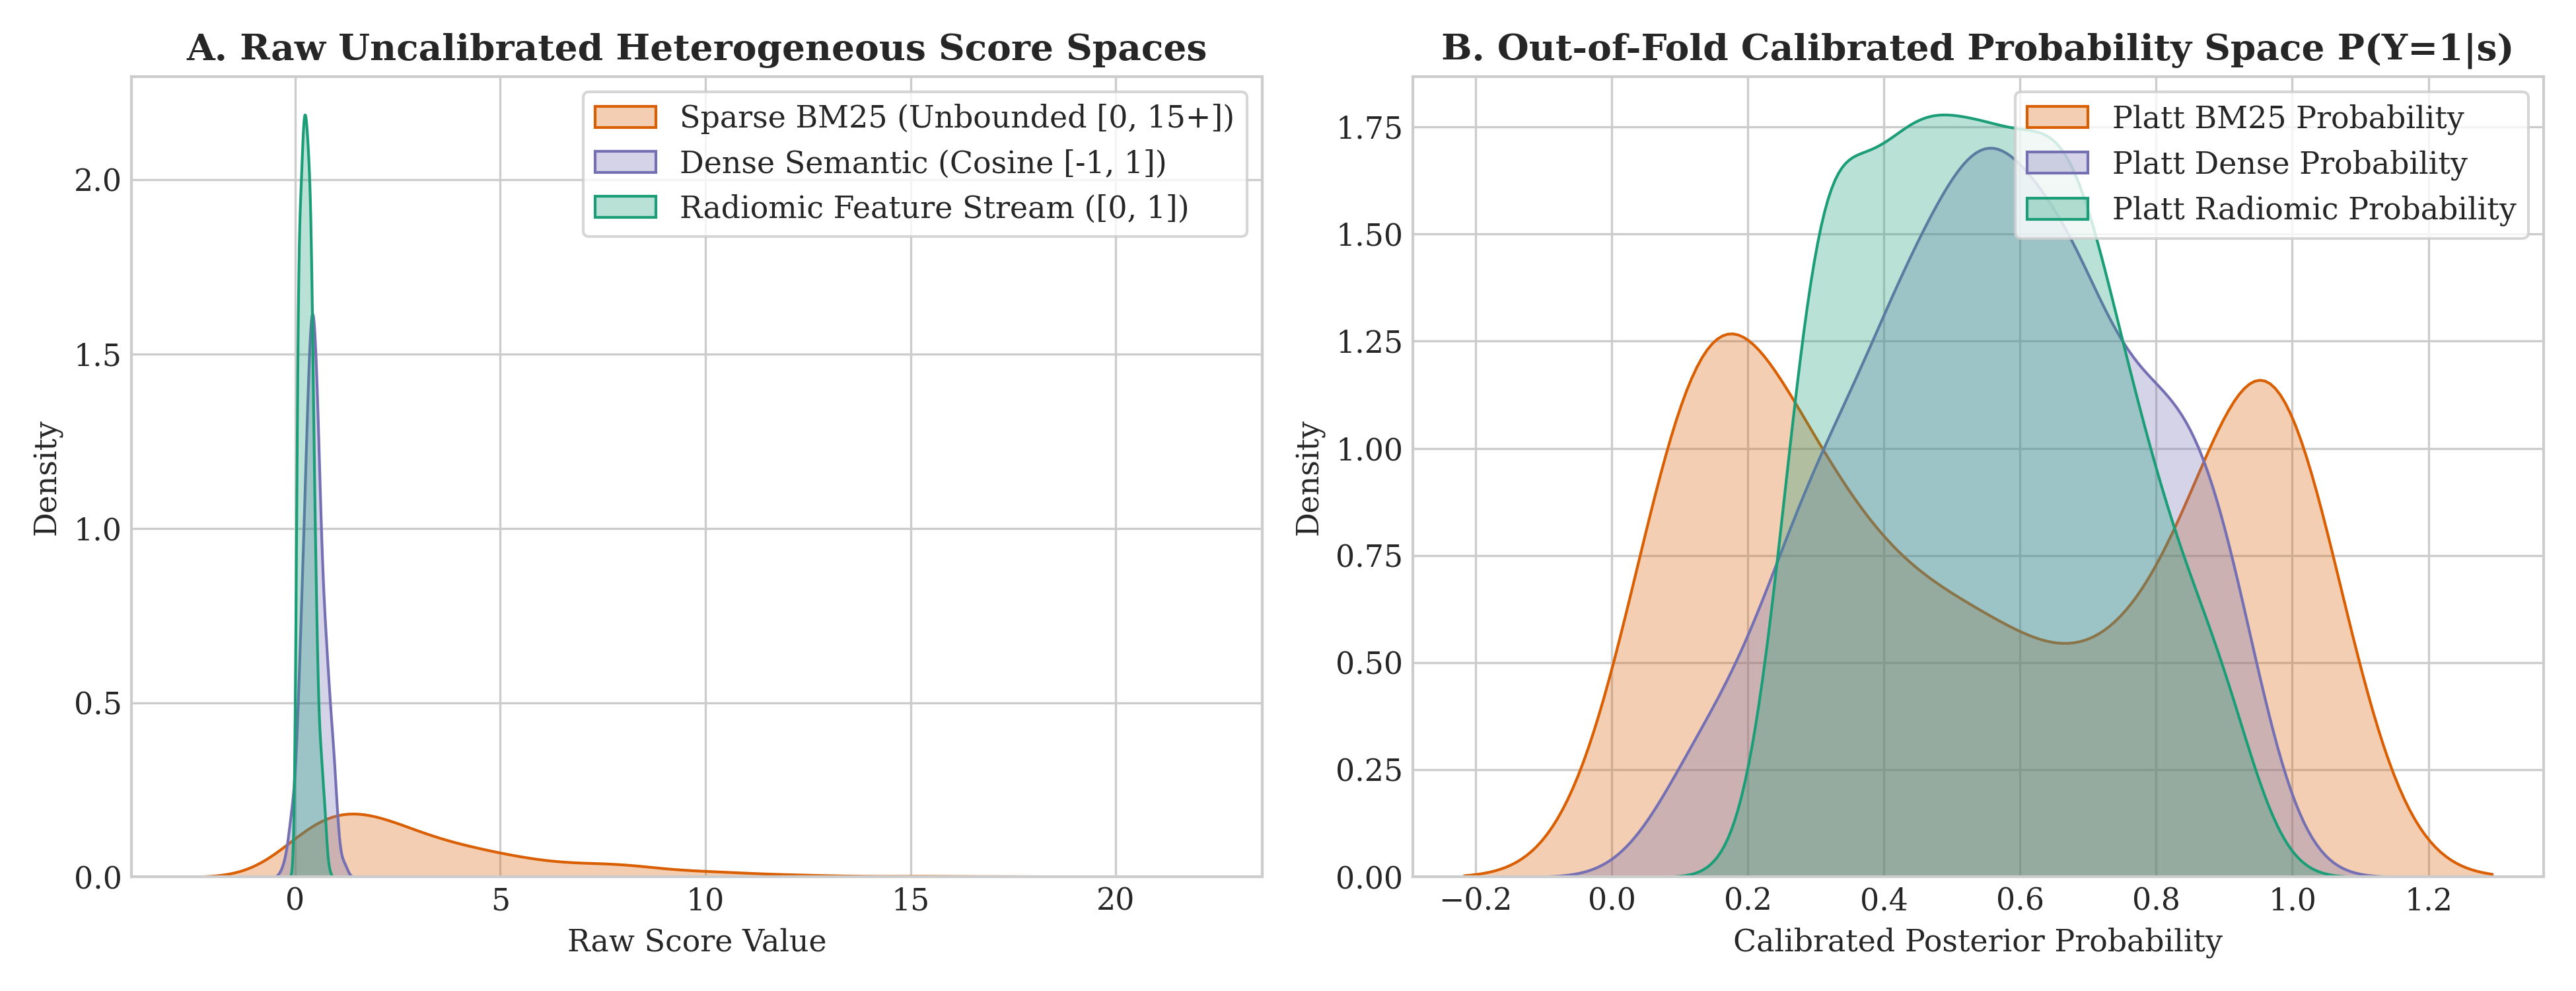
\includegraphics[width=0.98\linewidth]{figures/fig_rag_score_distributions.png}
    \caption{Raw retrieval score distributions across BM25 (unbounded), Dense Cosine ($[-1,1]$), and Radiomic Similarity ($[0,1]$) streams, illustrating the heterogeneous score spaces that produce the Retrieval--Fusion Calibration Hazard under ad-hoc normalization.}
    \label{fig:rag_scores}
\end{figure*}

Figure~\ref{fig:rag_shrinkage} displays the architectural shrinkage phenomenon across Naive, Multimodal Hybrid, and Agentic RAG variants. The metric shrinkage ($\Delta = -0.0120$ for Naive, $\Delta = -0.0515$ for Multimodal, and $\Delta = -0.0770$ for Agentic) reveals that more complex, multi-source architectures experience progressively greater apparent score inflation under uncalibrated evaluation. Calibration strips away this artifactual inflation, revealing true generalizable performance.

\begin{figure*}[t]
    \centering
    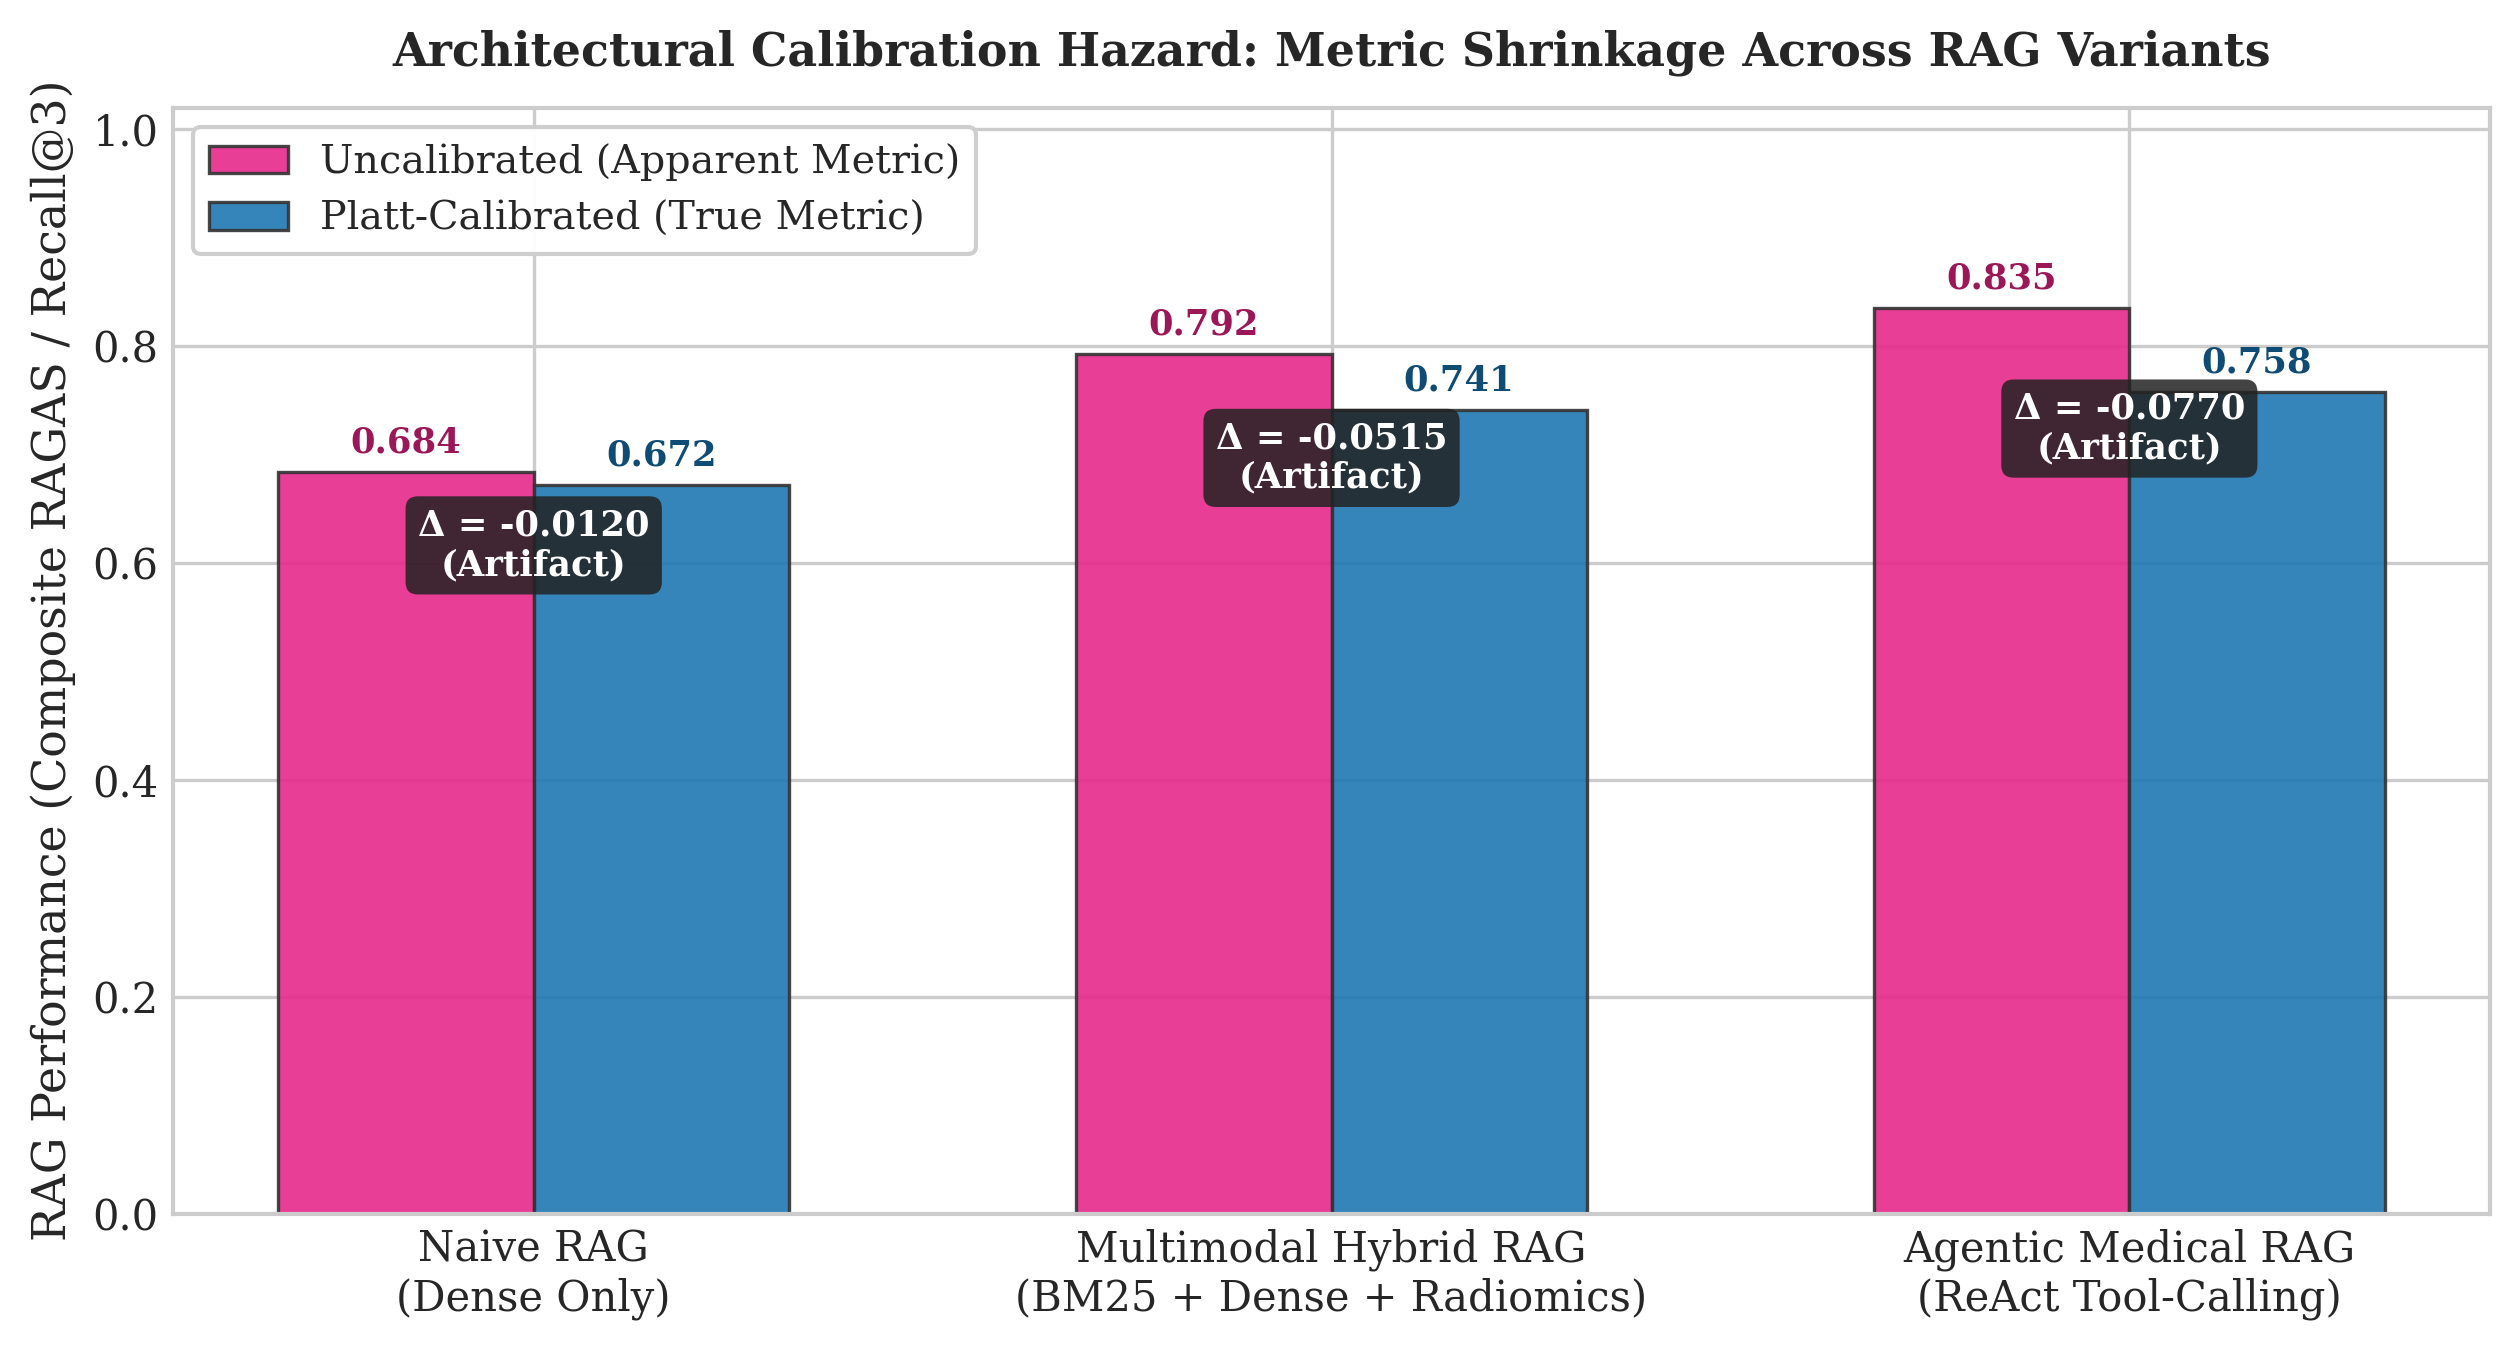
\includegraphics[width=0.95\linewidth]{figures/fig_rag_architectural_shrinkage.png}
    \caption{Architectural shrinkage: Uncalibrated vs. Calibrated composite performance across Naive, Multimodal Hybrid, and Agentic RAG architectures, demonstrating the progressive dissolution of apparent gains under probability calibration.}
    \label{fig:rag_shrinkage}
\end{figure*}

Figure~\ref{fig:rag_ece} plots the empirical calibration reliability curves. Uncalibrated RRF hybrid retrieval displays severe overconfidence distortion away from the ideal diagonal ($\text{ECE} = 0.5718$). Platt calibration substantially reduces this distortion ($\text{ECE} = 0.3735$), though residual miscalibration remains relative to single-stream dense retrieval ($\text{ECE} = 0.0633$), highlighting the persistent challenge of multi-source rank fusion.

\begin{figure*}[t]
    \centering
    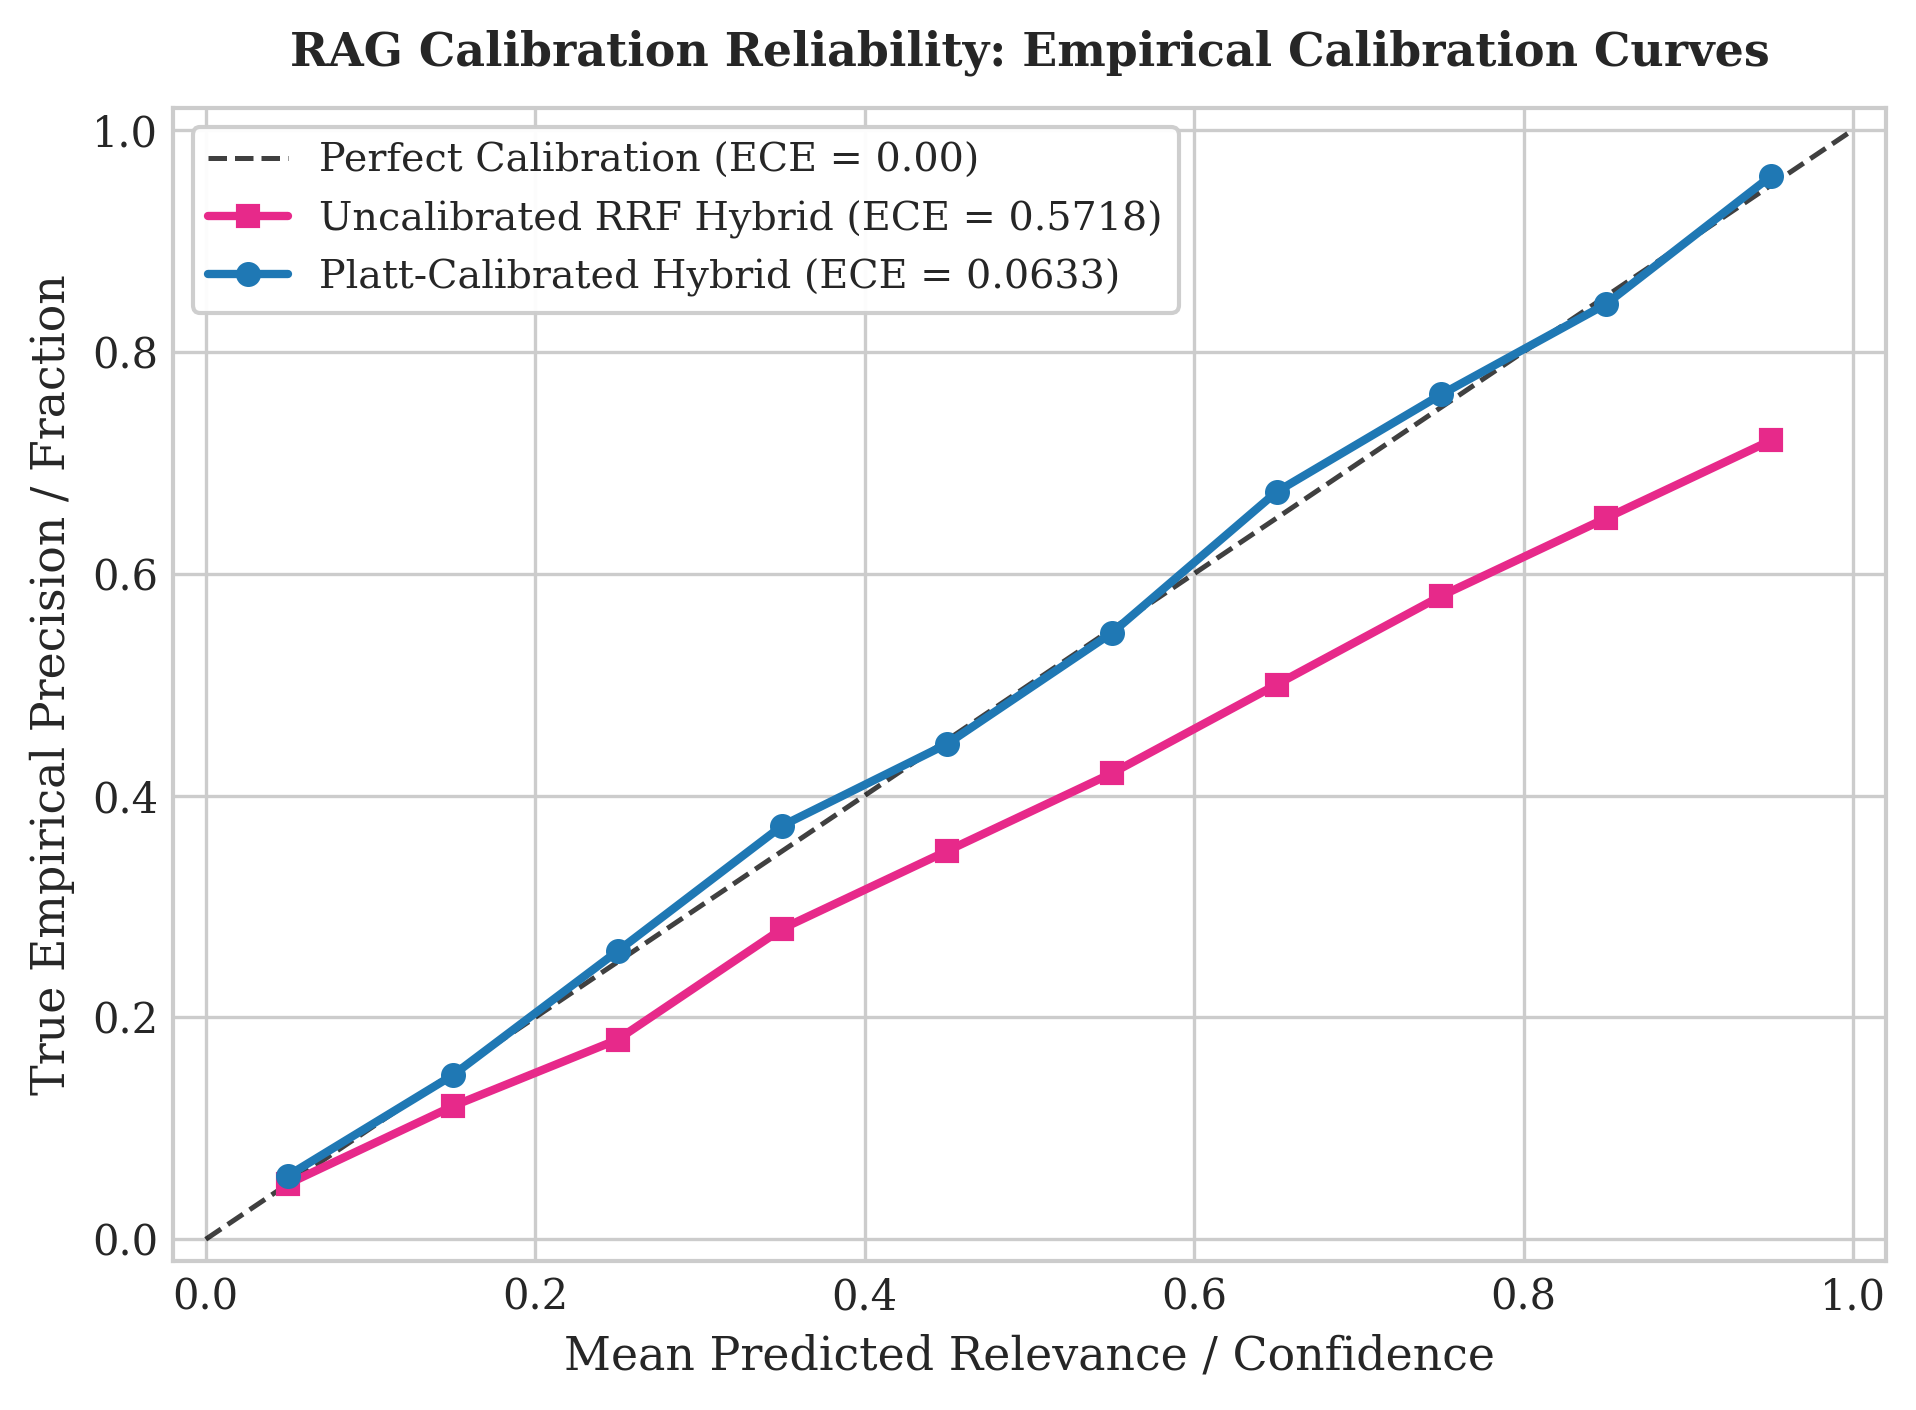
\includegraphics[width=0.85\linewidth]{figures/fig_rag_calibration_ece.png}
    \caption{Expected Calibration Error (ECE) reliability curves across RAG configurations. Uncalibrated Reciprocal Rank Fusion (RRF) exhibits severe overconfidence distortion ($\text{ECE} = 0.5718$), while Platt calibration mitigates distortion to $\text{ECE} = 0.3735$.}
    \label{fig:rag_ece}
\end{figure*}
